% =====================================================================
%  CONFERENCE VERSION -- 8 pages excluding references (CVPR / EarthVision).
%
%  ⚠️ THIS IS NOT A SECOND SOURCE OF TRUTH. It shares `numbers.tex` and
%  `refs.bib` with main.tex, so NO NUMBER CAN DIVERGE between the two:
%  change a value once and both papers change, or neither does.
%  `scripts/check_paper_consistency.py` enforces that and fails if either
%  file types a figure inline.
%
%  main.tex          -- the full version, no length target (journal/arXiv)
%  main_cvpr.tex     -- this file, cut to a conference limit
%  supplementary.tex -- shared overflow, cited by both
%
%  To submit: replace the two TEMPLATE lines with the venue class
%  (\usepackage{cvpr} or IEEEtran). Nothing else assumes a class.
% =====================================================================
\documentclass[10pt,twocolumn,letterpaper]{article}          % TEMPLATE
\usepackage[margin=1.9cm]{geometry}                          % TEMPLATE

\usepackage[T1]{fontenc}
\usepackage[utf8]{inputenc}
\usepackage{graphicx}
\usepackage{booktabs}
\usepackage{amsmath,amssymb}
\usepackage{multirow}
\usepackage{xcolor}
\usepackage[hidelinks]{hyperref}

\graphicspath{{../docs/}}
% =====================================================================
%  Every load-bearing number in the paper, defined ONCE.
%
%  WHY THIS FILE EXISTS. This project has caught five silent errors, and
%  the cheapest class of error left is a number that is right in the
%  results table and stale in the abstract. Macros make that impossible:
%  change it here and it changes everywhere, or it changes nowhere.
%
%  Each macro carries the file and section it came from. If a macro has
%  no citation it is not allowed in the paper.
% =====================================================================

% ---- baselines ------------------------------------------------------
\newcommand{\loveBase}{47.38}        % WEEK1 §5   reproduced, full val
\newcommand{\lovePub}{47.4}          % SegEarth-OV3, Table 1
\newcommand{\loveInstr}{47.37}       % WEEK1 §5   instrumented recompute (the gate)
\newcommand{\oemBase}{44.19}         % WEEK3 §7   384 of 500 val tiles
\newcommand{\oemPub}{42.9}           % SegEarth-OV3, published
\newcommand{\loveTiles}{1669}
\newcommand{\oemTiles}{384}

% ---- the residual ---------------------------------------------------
\newcommand{\discardPct}{29.68\%}    % WEEK1 §7.1
\newcommand{\discardPx}{323{,}184{,}908}
\newcommand{\discardOEM}{3.78\%}     % WEEK3 §7
\newcommand{\discardRatio}{3:1}      % WEEK1 §7.6  discard vs confusion
\newcommand{\mechA}{94.0\%}          % WEEK1 §7.7  below tau
\newcommand{\mechB}{6.0\%}           % WEEK1 §7.7  background won the argmax
\newcommand{\mechBpx}{19{,}378{,}177}
\newcommand{\mechBtiles}{24}
\newcommand{\mechBpots}{1.25\%}    % POTSDAM, reachability.py 4 Sep: argmax loss
\newcommand{\cnOemFloor}{0.1042}    % CONINFER_RESULTS: their OEM cache conf floor
\newcommand{\cnOemTau}{0.1}         % their published prob_thd on OpenEarthMap


% ---- the mechanism --------------------------------------------------
\newcommand{\bgShareLove}{36.1\%}    % WEEK3 §7
\newcommand{\bgShareOEM}{0.84\%}
\newcommand{\aucLove}{0.622}         % best of nine signals
\newcommand{\aucOEM}{0.913}          % conf2
\newcommand{\aucFloor}{0.53}         % empirical, size-stratified
\newcommand{\presCorrLove}{-0.750}
\newcommand{\presCorrOEM}{+0.094}
\newcommand{\catTilesLove}{198}
\newcommand{\catTilesOEM}{0}

% ---- refuted interventions -----------------------------------------
\newcommand{\tauCost}{-5.54}         % WEEK1 §7.2  tau 0.5 -> 0.1
\newcommand{\tauRatio}{1.73}         % WEEK1 §8.2  wrong per right
\newcommand{\presCost}{-11.97}       % WEEK1 §9.2b
\newcommand{\recoverLove}{+0.04}     % WEEK3 §8
\newcommand{\recoverOEM}{+2.28}      % WEEK3 §8   -- NEVER without \oemBgGain
\newcommand{\oemBgGain}{+22.67}      % WEEK3 §8.1
\newcommand{\oemRealLoss}{-2.11}     % WEEK3 §8.1
\newcommand{\oemBuildLoss}{-3.75}    % WEEK3 §8.1
\newcommand{\priorGain}{+0.2}        % WEEK3 §6   over a neighbour vote
\newcommand{\priorOracle}{+0.3}      % WEEK3 §6   with a PERFECT matrix

% ---- atomisation ----------------------------------------------------
\newcommand{\ceilCC}{72.8\%}         % WEEK3 §4
\newcommand{\ceilSLIC}{92.8\%}
\newcommand{\ceilSLICoem}{82.9\%}

% ---- the method -----------------------------------------------------
\newcommand{\methodGain}{+1.18}      % WEEK3 §9b  5-fold mean
\newcommand{\methodSD}{0.45}
\newcommand{\methodWorst}{+0.80}
\newcommand{\methodLand}{+8.30}      % 5-fold, six real classes
\newcommand{\methodBg}{-0.01}
\newcommand{\methodWater}{+6.78}
\newcommand{\methodWaterTau}{0.195}
\newcommand{\oracleBound}{+1.46}     % WEEK3 §9a  per-class oracle
\newcommand{\oracleShare}{81\%}
\newcommand{\globalOracle}{+0.04}    % WEEK3 §9a  best GLOBAL tau
\newcommand{\calibTiles}{200}        % WEEK3 §9b  every draw positive
\newcommand{\trainToVal}{-0.12}      % WEEK3 §9b  scope limit

% ---- end-to-end verification ---------------------------------------
\newcommand{\eeBase}{47.16}          % WEEK3 §9c  held-out tiles
\newcommand{\eeFit}{48.35}
\newcommand{\eeTiles}{1469}
\newcommand{\eeSpread}{0.175--0.675}

% ---- the label-free bound ------------------------------------------
\newcommand{\proxyBest}{+0.42}       % WEEK3 §9d  presence, best of eight
\newcommand{\proxyCtrl}{+0.58}       % random-control p95
\newcommand{\proxyConfRho}{+0.943}   % mean_conf vs precision
\newcommand{\proxyConfP}{0.017}
\newcommand{\proxyHeadRho}{+0.886}   % sem_inst_agree vs precision
\newcommand{\proxyHeadP}{0.033}
\newcommand{\proxyTauRho}{-0.429}    % precision vs ORACLE TAU -- the broken link
\newcommand{\proxyTauP}{0.419}
\newcommand{\nAttempts}{eleven}      % 3 threshold rules + 8 proxies

% ---- the co-occurrence prior ---------------------------------------
\newcommand{\pmiSignal}{0.574}       % ANALYSIS §4, corrected marginal
\newcommand{\pmiFloor}{0.003}
\newcommand{\pmiRatio}{216}
\newcommand{\rhoMined}{+0.757}       % WEEK3 §5  gate 1
\newcommand{\rhoCirc}{-0.257}        % circularity, retired

% ---- the confound stratification (WEEK3 §7a) -----------------------
\newcommand{\SHAREr}{42.9\%}       % LoveDA rural, catch-all share of GT
\newcommand{\SHAREu}{26.0\%}       % LoveDA urban
\newcommand{\CONFr}{25.5\%}        % rural confusability, measured
\newcommand{\CONFu}{43.3\%}        % urban -- the LOWER-share stratum is more confusable
\newcommand{\AUCr}{0.524}          % rural detection AUC (conf)
\newcommand{\AUCu}{0.730}          % urban

% ---- WEEK3_RESULTS.md 9e: per-class tau across LoveDA's domains -------------
\newcommand{\DOMr}{+2.77}          % rural within-domain gain, 5-fold
\newcommand{\DOMrsd}{0.92}
\newcommand{\DOMu}{+0.10}          % urban -- NOT distinguishable from zero (2/5 folds)
\newcommand{\DOMusd}{0.39}
\newcommand{\DOMrreal}{+18.61}     % rural, real classes aggregate
\newcommand{\DOMureal}{+4.18}      % urban, real classes aggregate -- land cover DOES gain
\newcommand{\DOMubg}{-3.51}        % urban catch-all pays for it: (4.18-3.51)/7 = +0.10
\newcommand{\DOMtaudiff}{0.227}    % mean |tau difference| between the domains
\newcommand{\DOMtaumax}{0.500}     % max, on `road' (0.725 rural vs 0.225 urban)
\newcommand{\DOMxr}{-0.40}         % mismatched -> rural, BELOW the published tau
\newcommand{\DOMxu}{-1.11}         % mismatched -> urban, BELOW the published tau
\newcommand{\DOMmr}{+2.32}         % matched -> rural, same 200-tile budget
\newcommand{\DOMmu}{+0.02}         % matched -> urban
\newcommand{\DOMpr}{+0.77}         % pooled -> rural: keeps a third of matched
\newcommand{\DOMpu}{-0.32}         % pooled -> urban

% ---- WEEK3_RESULTS.md 7b: the vocabulary intervention ----------------------
% det = max(AUC, 1-AUC). AUC is symmetric, so a raw AUC of 0.208 is a detector
% of strength 0.792 inverted, NOT an absent signal. Never quote raw AUC here.
\newcommand{\ivA}{0.794}           % A0, published vocabulary, det(conf)
\newcommand{\ivAtwo}{0.913}        % A0, det(conf2)
\newcommand{\ivShareA}{0.84\%}     % catch-all share, published
\newcommand{\ivShareD}{58.20\%}    % catch-all share, largest dose
\newcommand{\ivB}{0.582}           % faithful dose arm, det(conf)
\newcommand{\ivBtwo}{0.590}        % faithful dose arm, det(conf2)
\newcommand{\ivD}{0.710}           % arity-matched control, det(conf)
\newcommand{\ivDtwo}{0.855}        % arity-matched control, det(conf2)
\newcommand{\ivRatio}{2.5$\times$} % dose effect / control effect, conf
\newcommand{\ivRatioTwo}{5.6$\times$}  % ... conf2
\newcommand{\ivRatioWorst}{3.1$\times$} % conf2 vs the WORST control, not the matched one
\newcommand{\ivArms}{13}           % arms, all reading one cached score stack

% ---- WEEK3_RESULTS.md 7c: the reverse arm, and what bounds the mechanism ----
\newcommand{\ivRev}{0.540}         % LoveDA, catch-all removed from the VOCABULARY
\newcommand{\ivRevBase}{0.592}     % LoveDA A0 -- vocabulary change alone does nothing
\newcommand{\ivVocabMax}{0.052}    % largest move by ANY arm that leaves GT share alone
\newcommand{\ivSatShare}{35\%}     % above this, four points sit in one band
\newcommand{\ivSatLo}{0.58}
\newcommand{\ivSatHi}{0.64}

% ---- WEEK3_RESULTS.md 9f: no label-free rule for WHEN calibration pays ------
\newcommand{\crProxyRho}{+0.885}   % label-free catch-all fraction vs labelled discard, LoveDA
\newcommand{\crProxyRhoOEM}{+0.924}
\newcommand{\crLow}{$+2.13 \pm 0.18$}   % LEAST-residual stratum -- the most reliable gain
\newcommand{\crHigh}{$+3.22 \pm 3.15$}  % most-residual stratum -- worst fold -1.22
\newcommand{\crRho}{+0.400}        % LoveDA, over 4 strata
\newcommand{\crRhoOEM}{-0.500}     % OEM -- opposite sign, nothing replicates

% ---- WEEK3_RESULTS.md 9g: what the domain gap is made of --------------------
\newcommand{\cpWater}{48\%}        % water's share of the rural/urban gap
\newcommand{\cpForest}{37\%}       % forest's share
\newcommand{\cpTop}{85\%}          % the two together
\newcommand{\cpGapRho}{+0.713}     % P-R gap vs per-class delta IoU, 12 cells
\newcommand{\cpGapP}{0.013}        % permutation p
\newcommand{\cpPrecRho}{+0.168}    % precision ALONE -- explains nothing
\newcommand{\cpPrecP}{0.60}

% ---- WEEK3_RESULTS.md 9h: both metrics ------------------------------------
% ⚠️ ALWAYS the per-class MEAN (= catch-all-excluded mIoU), never the aggregate
% sum. Sections 9b/9e quote sums; +8.30 aggregate IS +1.38 here. Mixing them puts
% two numbers 6x apart in units next to each other.
\newcommand{\mrLoveFull}{+1.16}    % LoveDA, full mIoU, 5-fold held out
\newcommand{\mrLoveReal}{+1.36}    % LoveDA, catch-all-excluded mIoU
\newcommand{\mrLoveBg}{-0.02}
\newcommand{\mrOemFull}{+0.30}     % OEM, full mIoU -- looks flat
\newcommand{\mrOemReal}{+1.75}     % OEM, catch-all-excluded -- LARGER than LoveDA
\newcommand{\mrOemBg}{-11.30}
\newcommand{\mrOemLand}{+1.56}     % the real classes' contribution to full mIoU
\newcommand{\mrOemBgC}{-1.26}      % background's contribution: cancels it
\newcommand{\mrOemDistort}{3.38}   % OEM's baseline headline depression
\newcommand{\mrLoveLever}{14.3\%}  % 1/N -- the catch-all's share of the metric
\newcommand{\mrOemLever}{11.1\%}
\newcommand{\mrOemBgIoU}{17.13}
\newcommand{\methodLandMean}{+1.38}  % 9b's +8.30 aggregate, in mIoU units

% ---- CONINFER_RESULTS.md 7.1a: per-class tau on a CLIP backbone -------------
% ⚠️ Deltas measured on OUR reproduction (36.99), not their published 39.33. A
% delta is robust to a constant offset, but the text must say so.
\newcommand{\cnPub}{39.33}         % ConInfer's published LoveDA mIoU
\newcommand{\cnRepro}{36.99}       % our reproduction -- gap -2.34, full split
\newcommand{\cnGap}{2.34}          % CONINFER_RESULTS: repro below published
\newcommand{\cnTau}{0.8}           % THEIR published LoveDA threshold
\newcommand{\cnBase}{37.00}        % held-out baseline at their tau
\newcommand{\cnFit}{39.52}         % held out, per-class tau
\newcommand{\cnFull}{+2.52}
\newcommand{\cnReal}{+1.94}        % catch-all-excluded -- above SAM 3's +1.36
\newcommand{\cnBg}{+6.01}
\newcommand{\cnCV}{+2.51}          % five-fold mean
\newcommand{\cnCVsd}{0.34}
\newcommand{\cnWorst}{+2.22}       % every fold positive
\newcommand{\cnCalib}{25}          % tiles for a reliable gain -- 8x cheaper here
% ConInfer on OpenEarthMap: the transfer does NOT hold there, and why
\newcommand{\cnOemCV}{-0.39}       % five-fold, sd 1.28, 1/5 folds positive
\newcommand{\cnOemCVsd}{1.28}
\newcommand{\cnOemFull}{-0.09}
\newcommand{\cnOemReal}{+1.27}     % land cover DOES improve
\newcommand{\cnOemBg}{-10.94}      % catch-all sacrificed: 17.00 -> 6.06
\newcommand{\cnOemBgAfter}{6.06}
\newcommand{\mrOemBgAfter}{5.83}   % SAM 3 drives it to almost the same value

% ---- third dataset + the supervised-gap framing ----------------------------
\newcommand{\potsBase}{57.83}      % our Potsdam reproduction
\newcommand{\potsPub}{57.8}        % SegEarth-OV3 published -- matches to 0.03
\newcommand{\potsTiles}{2016}      % val tiles, 512^2, stride 512
% ⭐ The oracle is a fully supervised SegFormer-b0 with full training data,
% reported in SegEarth-OV3's own Table 2. Framing the gain as a share of the
% supervised gap is far more legible than a raw delta.
\newcommand{\oracleSup}{50.0}      % LoveDA, fully supervised
\newcommand{\gapClosed}{44\%}      % (48.53-47.37)/(50.0-47.37)

% ---- POTSDAM_RESULTS.md: the third dataset ---------------------------------
\newcommand{\potsShare}{4.29\%}    % `clutter` share of GT -- PRE-REGISTERED
\newcommand{\potsDiscard}{4.68\%}  % measured; committed bracket was 3.78-10.88%
\newcommand{\potsPoint}{4.5\%}     % the committed point estimate
\newcommand{\potsAuc}{0.578}       % best CACHED signal -- prediction was >0.622
% ⚠️ \aucLove is 0.622, LoveDA's best signal INCLUDING texture. For a like-for-like
% comparison with Potsdam (cached signals only) the LoveDA figure is 0.582.
\newcommand{\aucLoveCached}{0.582}
\newcommand{\aucOemCached}{0.794}
\newcommand{\potsReal}{+1.04}      % catch-all-excluded mIoU
\newcommand{\potsFull}{+0.59}      % five-fold full mIoU
\newcommand{\potsFullSd}{0.50}     % spread covers zero -- marginal, say so
\newcommand{\potsDistort}{8.18}    % clutter depresses the headline by this much

% ---------------------------------------------------------------------
%  THE SECOND LEVER: per-class scaling before the argmax.
%  ARGMAX_SCALING_RESULTS.md. All five-fold figures come from one script
%  (argmax_reorder.py) so the substitution table compares like with like.
% ---------------------------------------------------------------------
\newcommand{\scLove}{+1.16}          % LoveDA  C-B, 5-fold
\newcommand{\scLoveSD}{0.19}
\newcommand{\scLoveExcl}{+1.36}      % catch-all-excluded
\newcommand{\scLoveBg}{-0.03}
\newcommand{\scPots}{+4.86}          % Potsdam C-B, 5-fold
\newcommand{\scPotsSD}{0.35}
\newcommand{\scCI}{-0.10}            % ConInfer C-B, 5-fold
\newcommand{\scCISD}{0.14}
\newcommand{\scCIfolds}{1 of 5}
% the substitution table -- all five-fold, same script
\newcommand{\subCItau}{+2.51}
\newcommand{\subLovetau}{+1.16}
\newcommand{\subPotstau}{+0.59}
% end-to-end verification
\newcommand{\eeScaleLove}{+1.34}     % measured increment, LoveDA
\newcommand{\eeScaleLovePred}{+1.31}
\newcommand{\eePotsA}{57.60}
\newcommand{\eePotsB}{58.35}
\newcommand{\eePotsC}{63.27}
\newcommand{\eePotsScale}{+4.92}
\newcommand{\eePotsTotal}{+5.67}
\newcommand{\eePotsMiss}{0.05}       % worst rung miss vs prediction
\newcommand{\eePotsClassMiss}{0.23}  % worst per-class miss
% the tree case
\newcommand{\treeGap}{+54.7}
\newcommand{\treeP}{93.34}
\newcommand{\treeR}{38.63}
\newcommand{\treeTau}{+0.32}         % what per-class tau moved it
\newcommand{\treeScale}{+21.17}      % what the scale moved it, measured
\newcommand{\treeW}{3.73}
\newcommand{\scCalibPots}{100}
\newcommand{\confusionShare}{9.9\%}   % WEEK1 7.6: real-class confusion, LoveDA
\newcommand{\scSpread}{15\%}   % worst real-class fold spread, Potsdam (road)

% ---- the qualitative figure (scripts/fig_qualitative.py, Potsdam val) --------
% Row 4 is a tile where the method LOSES. It is in the figure deliberately: the
% five-fold Potsdam gain \scPots{} is an AVERAGE and four wins would misstate it.
\newcommand{\qualLoss}{7.72}         % 2_13_1024_0_1536_512, full mIoU 41.04->33.32
\newcommand{\qualLossRight}{26.1\%}  % of its changed pixels that became correct

% ---- the open-vocabulary run on Indian UAV imagery (scripts/fig_vocabulary.py)
% ⛔ NO GROUND TRUTH. These are per-class PIXEL SHARES with nodata excluded, not
% accuracy. Nothing derived from them may be phrased as a correctness claim.
\newcommand{\indTiles}{25}           % tiles cut from 5 OpenAerialMap scenes
\newcommand{\indScenes}{5}
\newcommand{\indGSD}{4--5\,cm}
\newcommand{\indFloodA}{78.6}        % `water` under the settlement vocabulary
\newcommand{\indFloodB}{79.1}        % `flood water` under the Indian one
\newcommand{\indBldgA}{18.2}         % `concrete roof`
\newcommand{\indBldgB}{18.3}         % `building`
\newcommand{\indVegA}{100.0}         % solar-farm tile collapses to ONE class
\newcommand{\indSolarB}{4.6}         % ⚠️ PARTIAL -- far below the panels' extent

% the tree case, absolute -- ARGMAX_SCALING_RESULTS.md, measured by eval.py on
% 1816 held-out Potsdam tiles. \treeScale is their difference.
\newcommand{\treeIoUa}{37.92}
\newcommand{\treeIoUb}{59.09}

% ---- combined totals, for the review presentation --------------------------
% Both levers together. LoveDA = \methodGain + \scLove ; Potsdam = eePotsC-eePotsA,
% measured end-to-end by eval.py, not summed from folds.
\newcommand{\loveTotal}{+2.32}       % 1.18 (tau) + 1.16 (scale), 5-fold
\newcommand{\potsTotal}{+5.67}       % 57.60 -> 63.27, eval.py, 1816 held-out tiles
\newcommand{\potsExcl}{+6.00}        % Potsdam catch-all-excluded, 5-fold

% ---- how much of the residual comes back -----------------------------------
% @DISCARD_AFTER_RESULTS.md, 12 Sep. scripts/discard_after.py, LoveDA full 1669
% tiles, 5-fold held out. The accounting identity
%   discard_A - discard_X == recovered - newly discarded
% is verified as exact integers on every run. Rates from a 40k px/tile
% subsample (42.9M real-class px scored); measure_discard_rate.py owns the
% absolutes at the published tau.
\newcommand{\raDiscA}{29.25\%}       % rung A, published tau
\newcommand{\raDiscB}{26.77\%}       % rung B, per-class tau
\newcommand{\raDiscC}{25.01\%}       % rung C, + per-class scale
\newcommand{\raDrop}{4.24}           % points, A -> C
\newcommand{\raRecov}{4.65\%}        % recovered vs A, rung C
\newcommand{\raNew}{0.40\%}          % newly discarded, rung C -- NEVER quote
                                     % \raRecov without this one (WEEK1 8.2)
\newcommand{\raCorrect}{79.2\%}      % of recovered, landing on the right class
\newcommand{\raWPR}{0.26}            % wrong per right, ours
\newcommand{\raTauCorrect}{36.6\%}   % of recovered, tau->0.1 = 1/(1+\tauRatio)
\newcommand{\raFactor}{6.6}          % \tauRatio / \raWPR
% per class, rung C. The four whose tau moved DOWN recover well; the two whose
% tau moved UP recover almost nothing and get it wrong -- by design.
\newcommand{\raWaterA}{31.9\%}
\newcommand{\raWaterC}{18.6\%}
\newcommand{\raWaterOk}{95.0\%}
\newcommand{\raRoadDelta}{+0.1}      % road DISCARDS MORE, deliberately

% ---- separability of the real objective ------------------------------------
% @SEPARABILITY_RESULTS.md. For a FIXED argmax a pixel predicted c either clears
% tau_c or becomes the catch-all -- never another real class -- so TP/FP/FN for
% class c depend on tau_c alone and the `real' objective is a sum of
% single-variable terms. Measured at exactly 0 on every class sweep.
\newcommand{\sepExact}{0.000000}     % max |delta tau| over all sweeps
\newcommand{\sepSweeps}{19}          % class-sweeps, LoveDA + Potsdam + OEM
\newcommand{\sepCostA}{$N\times201$} % cost of exact coordinate ascent
\newcommand{\sepCostB}{$201^{N}$}    % cost of the naive joint search
\newcommand{\sepAllMax}{0.0050}      % Potsdam, --objective all: it does NOT hold

% ---- how much of the oracle the fit captures -------------------------------
% Held-out real-class mIoU. Put this in limitations: it is a measured bound on
% the method, and naming it is stronger than letting a reader compute it.
\newcommand{\capLove}{83\%}
\newcommand{\capPots}{73\%}
\newcommand{\capOEM}{11\%}
\newcommand{\capOemWaterFit}{0.710}   % OEM water, fitted
\newcommand{\capOemWaterOra}{0.240}   % OEM water, oracle
\newcommand{\capOemWaterA}{69.18}     % its IoU at the oracle threshold
\newcommand{\capOemWaterB}{55.02}     % ... and at the fitted one

% ---- the one-standard-error rule: tested, and worse than what we deploy -----
\newcommand{\seLove}{+0.76}          % vs deployed +1.23
\newcommand{\sePots}{+0.55}          % vs deployed +0.90
\newcommand{\seOEM}{+0.54}           % vs deployed +0.28
\newcommand{\seMean}{-0.19}          % mean delta vs the deployed rule

% ---- which classes to calibrate: closed by an UPPER BOUND ------------------
% scripts/freeze_selection.py, LoveDA 1669 tiles, 5-fold held out.
\newcommand{\frzOracle}{+0.08}       % choosing on the EVALUATION fold
\newcommand{\frzCv}{-0.07}           % honest inner-CV selection

% ---- the five levers, one protocol ----------------------------------------
% Levers 1-2 reshape the DECISION and work; 3-5 are reported as bounded
% negatives. Every one was pre-registered.
\newcommand{\lvThreePots}{+0.04}     % head fusion, Potsdam
\newcommand{\lvThreeLove}{+0.22}     % head fusion, LoveDA
\newcommand{\lvFour}{+0.16}          % per-class presence weight, LoveDA
\newcommand{\lvFive}{-0.07}          % per-class bias (vector scaling), LoveDA
\newcommand{\lvFiveSD}{0.18}
\newcommand{\lvRhoCar}{2.33}         % Potsdam car -> instance head
\newcommand{\lvRhoBuild}{0.53}       % Potsdam building -> semantic head
\newcommand{\lvGammaRho}{+0.886}     % Spearman(median S_pres, gamma), p=0.017
\newcommand{\lvGammaP}{0.017}

% ---- sliding-window inference: tested, and it costs -------------------------
% @SLIDING_WINDOW_RESULTS.md. slide_crop=512, stride=341, LoveDA val 1669 tiles.
% SAM 3 resizes input to 1008^2, so 512^2 crops are UPSAMPLED ~2x -- the
% configuration the rest of this literature uses and SegEarth-OV3 does not.
% Precision RISES and recall COLLAPSES, which is a tighter gate rather than
% sharper features: S_pres is computed per view, so a class absent from a crop
% is vetoed there.
\newcommand{\swMIoU}{43.53}          % vs the published single-view 47.38
\newcommand{\swDelta}{-3.85}
\newcommand{\swPrec}{+1.1}           % mPrecision, single-view -> sliding-window
\newcommand{\swRec}{-4.7}            % mRecall
\newcommand{\swWater}{-14.28}        % water IoU, over half the total loss
\newcommand{\swWaterRec}{-16.1}      % water recall
\newcommand{\swBgRec}{+12.9}         % background recall: the catch-all absorbs MORE
\newcommand{\swCrop}{$512$}

% ---- and the gate was MITIGATING the loss, not causing it ------------------
% @SLIDING_WINDOW_RESULTS.md 2a. Loosening the presence gate under sliding
% window costs MORE, and precision collapses while recall barely moves -- so the
% per-crop veto was suppressing false positives, not valid predictions.
\newcommand{\swMax}{39.86}           % gate = max presence over crops
\newcommand{\swGlobal}{39.05}        % gate = one whole-image forward
\newcommand{\swMaxDelta}{-3.67}      % vs the per-crop gate
\newcommand{\swPrecDrop}{68.1 \rightarrow 58.2 \rightarrow 56.7}
\newcommand{\swBuildPrec}{77.0 \rightarrow 49.4}

% ---- dihedral test-time augmentation --------------------------------------
% @TTA_RESULTS.md. Average the score stacks over flipped/rotated views of the
% WHOLE image -- unlike crops, the field of view and therefore the presence
% semantics are identical across views, which is why this works where sliding
% window did not. Aerial imagery has no canonical orientation, so the argument
% is specific to remote sensing.
\newcommand{\ttaHflip}{47.67}        % 2 views, LoveDA val 1669 tiles
\newcommand{\ttaHflipD}{+0.29}
\newcommand{\ttaDfour}{47.84}        % 8 views (all dihedral transforms)
\newcommand{\ttaDfourD}{+0.47}
\newcommand{\ttaPrec}{+0.4}          % mPrecision, hflip -- BOTH rise, uniquely
\newcommand{\ttaRec}{+0.1}           % mRecall
\newcommand{\ttaCost}{6.59}          % s/image at 8 views vs 0.85 baseline
% ⭐ Paired fold-by-fold, same 800 tiles / seed / fold partition. TTA's gain at
% each rung: it survives per-class tau and is ABSORBED by the per-class scale,
% because both change which class wins the argmax.
\newcommand{\ttaAtA}{+0.42}
\newcommand{\ttaAtB}{+0.58}
\newcommand{\ttaAtC}{+0.06}
\newcommand{\ttaScaleWith}{+0.74}    % lever 2's own gain WITH tta
\newcommand{\ttaScaleWithout}{+1.26} % ... and without

% =====================================================================
%  UAVid — the fourth dataset.  @UAVID_RESULTS.md
% =====================================================================
\newcommand{\uavPub}{54.7}           % SegEarth-OV3 Table 2, UAVid^img
\newcommand{\uavBase}{56.86}         % UAVID §1   our reproduction, their vocabulary
\newcommand{\uavGap}{+2.16}          % UAVID §1   unexplained
\newcommand{\uavTiles}{70}           % official val frames
\newcommand{\uavTrainTiles}{200}     % official train frames (real, excl. augmented)
\newcommand{\uavScenes}{20}          % flights in the train split
\newcommand{\uavValScenes}{7}        % flights in the val split
\newcommand{\uavOracle}{59.7}        % their supervised SegFormer-b0 row
\newcommand{\uavCatchShare}{16.16\%} % UAVID §4   catch-all share of GT
\newcommand{\uavDiscard}{6.81\%}     % UAVID §1   real-class pixels to catch-all

% ---- levers on UAVid, group-disjoint folds --------------------------
\newcommand{\uavTauCV}{+1.34}        % UAVID §12  5-fold, 20 flights
\newcommand{\uavTauSD}{0.39}
\newcommand{\uavTauWorst}{+0.75}
\newcommand{\uavScaleCV}{+5.89}      % UAVID §16  5-fold, on top of lever 1
\newcommand{\uavScaleSD}{1.51}
\newcommand{\uavOracleBound}{+1.40}  % UAVID §16  per-class tau oracle, 200 frames

% ---- transfer: fitted on train, applied unchanged to val ------------
\newcommand{\uavTauTrans}{+1.03}     % UAVID §14  lever 1 across the split
\newcommand{\uavTauTransPerm}{0.0\%} % shuffles matching it
\newcommand{\uavScaleTrans}{+5.64}   % UAVID §17  lever 2 across the split
\newcommand{\uavScalePerm}{1.0\%}
\newcommand{\uavScaleShuffle}{-2.82} % UAVID §20  shuffled assignment, corrected prompt
\newcommand{\uavCalibScenes}{3}      % UAVID §14  scenes for +0.81
\newcommand{\uavCalibGain}{+0.81}

% ---- verified end-to-end --------------------------------------------
\newcommand{\uavEEone}{57.92}        % UAVID §15  eval.py, lever 1
\newcommand{\uavEEtwo}{63.55}        % UAVID §18  eval.py, lever 1 + lever 2
\newcommand{\uavEEpred}{63.55}       % cached prediction -- agrees exactly
\newcommand{\uavEEmax}{0.20}         % largest per-class disagreement
\newcommand{\uavaAccA}{79.24}        % UAVID §18  pixel accuracy, baseline
\newcommand{\uavaAccC}{84.81}
\newcommand{\uavPrecD}{+0.60}        % mPrecision, lever 1+2 vs baseline
\newcommand{\uavRecD}{+4.92}         % mRecall

% ---- the corrected configuration -------------------------------------
\newcommand{\uavCorrBase}{60.40}     % UAVID §19  with `low vegetation'
\newcommand{\uavCorrOne}{+1.19}      % lever 1 on the corrected prompt
\newcommand{\uavCorrTwo}{+2.03}      % lever 2 on the corrected prompt
\newcommand{\uavCorrMethod}{+3.22}   % UAVID §20  the honest method contribution
\newcommand{\uavCorrFinal}{63.62}
\newcommand{\uavScaleLost}{64\%}     % share of lever 2's gain the prompt took

% =====================================================================
%  The vocabulary.  @VOCABULARY_RESULTS.md  -- pre-registered, two arms
% =====================================================================
\newcommand{\vocUavGain}{+3.53}      % VOCAB §1   vegetation -> low vegetation
\newcommand{\vocUavTree}{+14.66}     % tree IoU
\newcommand{\vocUavVeg}{+11.14}      % low-vegetation IoU
\newcommand{\vocUavElse}{0.04}       % largest move among the other real classes
\newcommand{\vocUavVegPrecA}{53.62}
\newcommand{\vocUavVegPrecB}{71.51}
\newcommand{\vocUavTreeRecA}{55.90}
\newcommand{\vocUavTreeRecB}{72.76}
\newcommand{\vocPotsBase}{57.83}     % VOCAB §2   recorded Potsdam baseline
\newcommand{\vocPotsNew}{55.12}      % with `low vegetation'
\newcommand{\vocPotsGain}{-2.71}
\newcommand{\vocPotsTreeRec}{38.63}  % IDENTICAL before and after
\newcommand{\vocPotsTreePrecA}{93.34}
\newcommand{\vocPotsTreePrecB}{92.17}
\newcommand{\vocLoveBarren}{+4.94}   % PROMPT_ENSEMBLE, LoveDA `barren'
\newcommand{\vocRouteA}{63.55}       % UAVID §20  bad prompt + both levers
\newcommand{\vocRouteB}{63.62}       % one word + both levers
\newcommand{\vocRouteDelta}{0.07}

% ---- the data traps, reported in setup -------------------------------
\newcommand{\uavLeak}{+0.54}         % UAVID §8   frame-level folds inflate lever 1
\newcommand{\uavLeakA}{+1.05}        % leaking
\newcommand{\uavLeakB}{+0.51}        % group-disjoint
\newcommand{\uavAug}{400}            % augmented copies shipped among 600 `train' frames
\newcommand{\uavFrames}{10}          % consecutive frames per flight

% ---- values that were typed inline until the consistency check caught them ----
% ⚠️ \waterRec is 54.7 and \uavPub is ALSO 54.7 -- water's recall and UAVid's
% published mIoU are unrelated. Never reuse a macro because the value matches.
\newcommand{\tauLove}{0.5}           % published thresholds, per dataset
\newcommand{\tauOEM}{0.1}
\newcommand{\tauPots}{0.1}
\newcommand{\tauUav}{0.3}
\newcommand{\waterPrec}{89.5}        % WEEK1 §5  LoveDA water, the motivating asymmetry
\newcommand{\waterRec}{54.7}
\newcommand{\eeSpreadHi}{0.675}      % WEEK3 §9c fitted span, high end (\eeSpread = low)
\newcommand{\bndWaterPrec}{88.5}     % WEEK3 §9d precision vs oracle tau, non-monotone
\newcommand{\bndRoadPrec}{68.5}
% ⚠️ \oemTauCV is +0.16 and \lvFour is ALSO +0.16 -- OpenEarthMap's threshold gain
% and lever four's null. The second value collision this check caught; matching on
% a value rather than a meaning would have put the wrong citation in the paper.
\newcommand{\oemTauCV}{+0.16}        % WEEK3 §9b OpenEarthMap, 5-fold, full mIoU
\newcommand{\oemTauSD}{0.93}

% =====================================================================
%  DLRSD -- the fifth dataset, and the only one with NO catch-all.
%  @DLRSD_RESULTS.md.  Added 19 Sep 2026; nothing here appears in the
%  paper body yet.
% =====================================================================
\newcommand{\dlrTiles}{2100}         % DLRSD §2  images, 256 x 256
\newcommand{\dlrHeld}{1701}          % DLRSD §1  held-out tiles
\newcommand{\dlrCalib}{399}          % DLRSD §1  calibration draw, stratified
\newcommand{\dlrClasses}{17}
\newcommand{\dlrCatchShare}{0.00\%}  % DLRSD §2  no catch-all class exists
\newcommand{\dlrDiscard}{6.16\%}     % DLRSD §5  real-class pixels to the sink
% ---- the three verified rungs (eval.py, published vocabulary) --------
\newcommand{\dlrEEa}{37.27}          % DLRSD §1  baseline, published tau = 0.1
\newcommand{\dlrEEb}{39.04}          % + per-class tau
\newcommand{\dlrEEc}{44.42}          % + per-class scale
\newcommand{\dlrTotal}{+7.15}
% ---- five-fold, the figures with an error bar -----------------------
\newcommand{\dlrTauCV}{+2.37}        % DLRSD §7  lever 1
\newcommand{\dlrTauSD}{0.63}
\newcommand{\dlrScaleCV}{+5.84}      % DLRSD §8  lever 2 on top of lever 1
\newcommand{\dlrScaleSD}{1.03}
% ---- the oracle: one threshold against seventeen --------------------
\newcommand{\dlrOracleGlobal}{+0.04} % DLRSD §6  best POSSIBLE single tau
\newcommand{\dlrOraclePer}{+2.99}    % best per-class tau
% ---- pixel accuracy, so the mean cannot be dismissed as class averaging
\newcommand{\dlraAccA}{58.94}        % DLRSD §9  eval.py, baseline
\newcommand{\dlraAccC}{65.79}        % both levers
% ---- the vocabulary arm, its own result -----------------------------
\newcommand{\dlrVocBase}{+1.71}      % DLRSD §13 corrected words, before the levers
\newcommand{\dlrVocAfter}{+1.70}     % after them -- the two ADD
\newcommand{\dlrVocEEc}{46.12}       % best verified configuration
% ---- the honest per-class costs -------------------------------------
\newcommand{\dlrWaterLoss}{-2.73}    % DLRSD §9  worst class, under BOTH levers
\newcommand{\dlrTilesUp}{1057}       % DLRSD §10b per-tile outcome
\newcommand{\dlrTilesDown}{769}
\newcommand{\dlrTilesDead}{22}       % emptied entirely -- a stated failure mode
\newcommand{\dlrLeverage}{35.3\%}    % share of the metric owned by classes under 2% of pixels

% =====================================================================
%  The class-scale SEARCH RANGE -- an unreported hyperparameter, measured
%  on four datasets.  @ARGMAX_SCALING_RESULTS.md, 18 Sep 2026.
%  The method's range is 0.40--2.50; these are the sensitivity figures.
% =====================================================================
\newcommand{\rangeLo}{0.40}
\newcommand{\rangeHi}{2.50}
\newcommand{\rangeWideLo}{0.10}
\newcommand{\rangeWideHi}{10}
\newcommand{\rangeDlr}{+1.04}        % wide minus default, DLRSD  (+5.84 -> +6.88)
\newcommand{\rangePots}{+0.66}       % Potsdam (+4.86 -> +5.52)
\newcommand{\rangeLove}{-0.19}       % LoveDA  (+1.16 -> +0.97) and the fit destabilises
\newcommand{\rangeUav}{-0.24}        % UAVid   (+5.89 -> +5.65)
\newcommand{\rangeLoveSDa}{0.19}     % LoveDA fold sd, default range
\newcommand{\rangeLoveSDb}{0.75}     % ... wide range: four times larger
\newcommand{\rangeLoveSpread}{144.7\%} % fitted scales across folds, wide range
\newcommand{\rangeDlrEE}{45.52}      % DLRSD, wide range, verified by eval.py
\newcommand{\rangeDlraAcc}{63.66}    % ... and its pixel accuracy: 65.79 -> 63.66
\newcommand{\rangePotsEE}{63.82}     % Potsdam, wide range, verified


\newcommand{\best}[1]{\textbf{#1}}
\newcommand{\bg}{\texttt{background}}
\newcommand{\suppref}[1]{the supplementary material}

\title{Calibrating the Decision, Not the Model:\\
       Per-Class Thresholds for Training-Free Open-Vocabulary
       Remote-Sensing Segmentation}

\author{%
  Priyanshu Kumar, \quad Raj Gautam, \quad Shounak Chakraborty, \quad K.~Sathya Babu\\[2pt]
  Indian Institute of Information Technology Design and Manufacturing, Kurnool\\
  \texttt{\{123cs0045, 123ad0059, shounak, ksb\}@iiitk.ac.in}%
}
\date{}

\begin{document}
\maketitle

\begin{abstract}
Training-free open-vocabulary segmentation pipelines built on SAM~3 gate their
predictions with a single confidence threshold and assign everything below it to a
\bg{} class. On LoveDA this discards \discardPct{} of all real-class pixels
(\discardPx{}), with silence outnumbering misclassification \discardRatio{}. We show
the single threshold is the wrong \emph{shape} for the problem, and that two
corrections recover a substantial part of what it costs --- one threshold per class,
and one multiplier per class applied before the argmax --- both fitted on
\calibTiles{} labelled tiles with no weights trained, the same supervision the
baseline already spends tuning its one threshold. Per-class thresholds give
\methodGain{}~$\pm$~\methodSD{}~mIoU on LoveDA, \uavTauCV{}~$\pm$~\uavTauSD{} on
UAVid, and \cnCV{}~$\pm$~\cnCVsd{} on a CLIP-based competitor at its own operating
point, so the correction composes with prior work rather than competing with it. The
multiplier reaches errors no threshold can, because it changes which class wins:
Potsdam's \texttt{tree} gains \treeScale{}~IoU where thresholds move it \treeTau{}.
All results are verified in the unmodified evaluation pipeline. We then report a
finding that limits our own: \best{the hand-written prompt list every training-free
method inherits is a larger lever than the method.} Replacing one word with a
dataset's own class name is worth \vocUavGain{}~mIoU on UAVid --- more than our
complete method earns on LoveDA --- and removes \uavScaleLost{} of the multiplier's
gain there, so we restate that dataset's contribution as \uavCorrMethod{}. The same
rule applied to Potsdam \emph{costs} \vocPotsGain{}~mIoU. No lookup rule exists, and
no compared method reports its prompts. Finally, \nAttempts{} label-free rules fail
to reach the oracle bound, four of which provably estimate per-class precision: the
optimal threshold solves a \emph{coupled} multi-class objective that no per-class
statistic can express, so the labelled calibration set is irreducible.
\end{abstract}

% =====================================================================
\section{Introduction}
\label{sec:intro}

A training-free open-vocabulary segmenter is handed a list of class names and asked
to label every pixel without seeing an annotation. The dominant recipe for remote
sensing scores each class independently, takes an argmax, and then applies one global
confidence threshold: pixels below it become \bg{}. The threshold is not incidental.
It is tuned per dataset by its authors, on labelled data, and published as part of the
configuration --- $\tauLove{}$ on LoveDA, $\tauOEM{}$ on OpenEarthMap, $\tauUav{}$ on UAVid.

We begin from what that one number costs. Reproducing the strongest published SAM~3
pipeline at \loveBase{}~mIoU on LoveDA against its reported \lovePub{}, we measure
that \discardPct{} of every pixel carrying a real land-cover label is assigned to
\bg{} --- \discardPx{} pixels --- and that this silence outnumbers outright
misclassification \discardRatio{}. The obvious remedy fails: sweeping the threshold
down to $\tauOEM{}$ recovers two thirds of that mass at a cost of \tauRatio{} wrong pixels
for every right one, and \best{loses} mIoU.

\paragraph{The claim.} A single confidence threshold is the wrong shape for a
multi-class decision, because different classes are wrong in different directions.
\texttt{water} on LoveDA is right $\waterPrec{}\%$ of the times it fires and finds only
$\waterRec{}\%$ of what is there; \texttt{road} is the reverse. One number cannot serve
both, and the fitted values span $\eeSpread{}$ to $\eeSpreadHi{}$ where the published one is $\tauLove{}$
for all of them. Fitting one threshold per class on \calibTiles{} labelled tiles ---
\best{no weights trained, and the same protocol the baseline already uses for its
single threshold} --- recovers \methodGain{}~$\pm$~\methodSD{}~mIoU.

Per-class thresholds are provably the \emph{complete} family of corrections available
after the argmax (Sec.~\ref{sec:method}). That result is what motivates the second
lever: if nothing more can be done after the argmax, the remaining freedom is
\emph{at} it. We fit one multiplier per class applied to the scores before the argmax,
with the threshold still reading the raw score, and it reaches an error mass no
threshold can touch --- a pixel whose correct class lost the argmax cannot be
recovered by lowering that class's bar.

\paragraph{And a finding that limits our own.} Every method in this literature
inherits a hand-written list of class prompts, and none report how it was chosen.
We tested two, each with the prediction registered before the run. Replacing UAVid's
\texttt{vegetation} --- a word that also names trees --- with the dataset's own term
\emph{low vegetation} is worth \vocUavGain{}~mIoU and removes \uavScaleLost{} of our
second lever's gain there. The identical rule applied to Potsdam \best{costs}
\vocPotsGain{}. \best{The vocabulary is the largest single lever we measure, its
direction is not predictable, and it is unreported.}

\paragraph{Contributions.}
\begin{enumerate}\itemsep2pt
  \item \textbf{A method, and a completeness result that bounds it.} Per-class
        thresholds give \methodGain{}~$\pm$~\methodSD{} on LoveDA, \uavTauCV{} on
        UAVid and \cnCV{} on a CLIP pipeline, all verified end to end. Any per-class
        monotone recalibration composed with a global threshold reduces to this rule
        exactly (Sec.~\ref{sec:method}).
  \item \textbf{A second lever, motivated by that bound.} A per-class scale before
        the argmax adds \scPots{}~$\pm$~\scPotsSD{} on Potsdam, \scLove{} on LoveDA
        and \uavScaleCV{} on UAVid over thresholds alone. It reaches Potsdam's
        \texttt{tree}, which has the largest precision--recall gap we measure
        (\treeGap{}) and which thresholds move \treeTau{}.
  \item \textbf{\best{A larger lever than either, and a correction to our own
        result.}} One word is worth \vocUavGain{} on UAVid and \vocLoveBarren{} on
        LoveDA against \loveTotal{} for our complete method; the same rule costs
        \vocPotsGain{} on Potsdam (Sec.~\ref{sec:vocab}).
  \item \textbf{A reporting recommendation.} We observe a catch-all class moving the
        headline mIoU in both directions and recommend reporting mIoU over the real
        classes beside it.
  \item \textbf{A bound with its reason.} \nAttempts{} label-free rules fail; four
        provably estimate per-class precision, which we had supposed was the missing
        quantity. It is not.
\end{enumerate}

% =====================================================================
\section{Related work}
\label{sec:related}

Dense open-vocabulary segmentation from CLIP begins with MaskCLIP~\cite{maskclip} and
continues through SCLIP~\cite{sclip}, ClearCLIP~\cite{clearclip} and
ProxyCLIP~\cite{proxyclip}, each removing an obstacle between CLIP's image-level
training and pixel-level use. SegEarth-OV~\cite{segearthov} adapts that line to
remote sensing with a feature upsampler, and SegEarth-OV3~\cite{segearthov3} replaces
the stack with SAM~3~\cite{sam3}, fusing a semantic and an instance head and gating by
a presence score. That pipeline is our baseline and we reproduce it.

ConInfer~\cite{coninfer} is the nearest competitor: it fits a per-scene visual prior
over DINOv3 features and fuses it with a VLM posterior, and reports gains over
SegEarth-OV on the same benchmarks. It is orthogonal to us --- it changes the
\emph{scores}, we change the \emph{decision rule} applied to them --- and we show the
two compose.

Our corrections are recalibration in the sense of Guo~\etal~\cite{guo2017} and
Kull~\etal~\cite{kull2019}, but applied to a decision rather than to a probability:
we never ask the scores to be calibrated, only that the rule reading them be
class-aware. What we add to that literature is a completeness argument for the
post-argmax family and a measured demonstration that the remaining freedom lies at
the argmax itself.

% =====================================================================
\section{Setup}
\label{sec:setup}

We evaluate on four segmentation benchmarks and one competing pipeline. LoveDA
(\loveTiles{} validation tiles) and OpenEarthMap (\oemTiles{} of the official 500)
are land-cover benchmarks; Potsdam is ISPRS aerial imagery at \best{5\,cm} ground
sampling distance; UAVid is low-altitude drone video, a different sensor and
viewpoint from the other three. We reproduce the published baseline on each:
\loveBase{} against \lovePub{} on LoveDA, \potsBase{} against \potsPub{} on Potsdam,
\oemBase{} against \oemPub{} on OpenEarthMap, and \uavBase{} against \uavPub{} on
UAVid. The last differs by \uavGap{} under identical code, configuration, vocabulary
and thresholds, and we report both figures rather than explain it away
(Sec.~\ref{sec:limitations}).

\paragraph{Two properties of UAVid change the protocol.} Its validation split is
\uavValScenes{} drone flights of \uavFrames{} \emph{consecutive} frames, so a
frame-level cross-validation places near-duplicates of every evaluation frame in the
calibration set: it reports \uavLeakA{} where the flight-grouped answer is
\uavLeakB{}, \best{a leak worth \uavLeak{}~mIoU that flips two of five folds}. Its
distributed training split further ships \uavAug{} flipped and shifted copies among
$600$ frames. All UAVid results here group folds by flight and exclude the augmented
copies. We report both because neither is visible in the directory structure and both
produce a clean, plausible, wrong number.

\paragraph{Protocol.} Thresholds and scales are fitted by coordinate ascent on a
calibration subset and evaluated on disjoint tiles, with the published-threshold
baseline recomputed on the same held-out pixels. The fit maximises mIoU over the real
classes only; full mIoU is still what we report. Every headline is verified by running
the fitted parameters through the unmodified evaluation pipeline, not only through the
cached statistic used to search.

% =====================================================================
\section{What the baseline discards, and what governs it}
\label{sec:mechanism}

\begin{figure*}[t]\centering
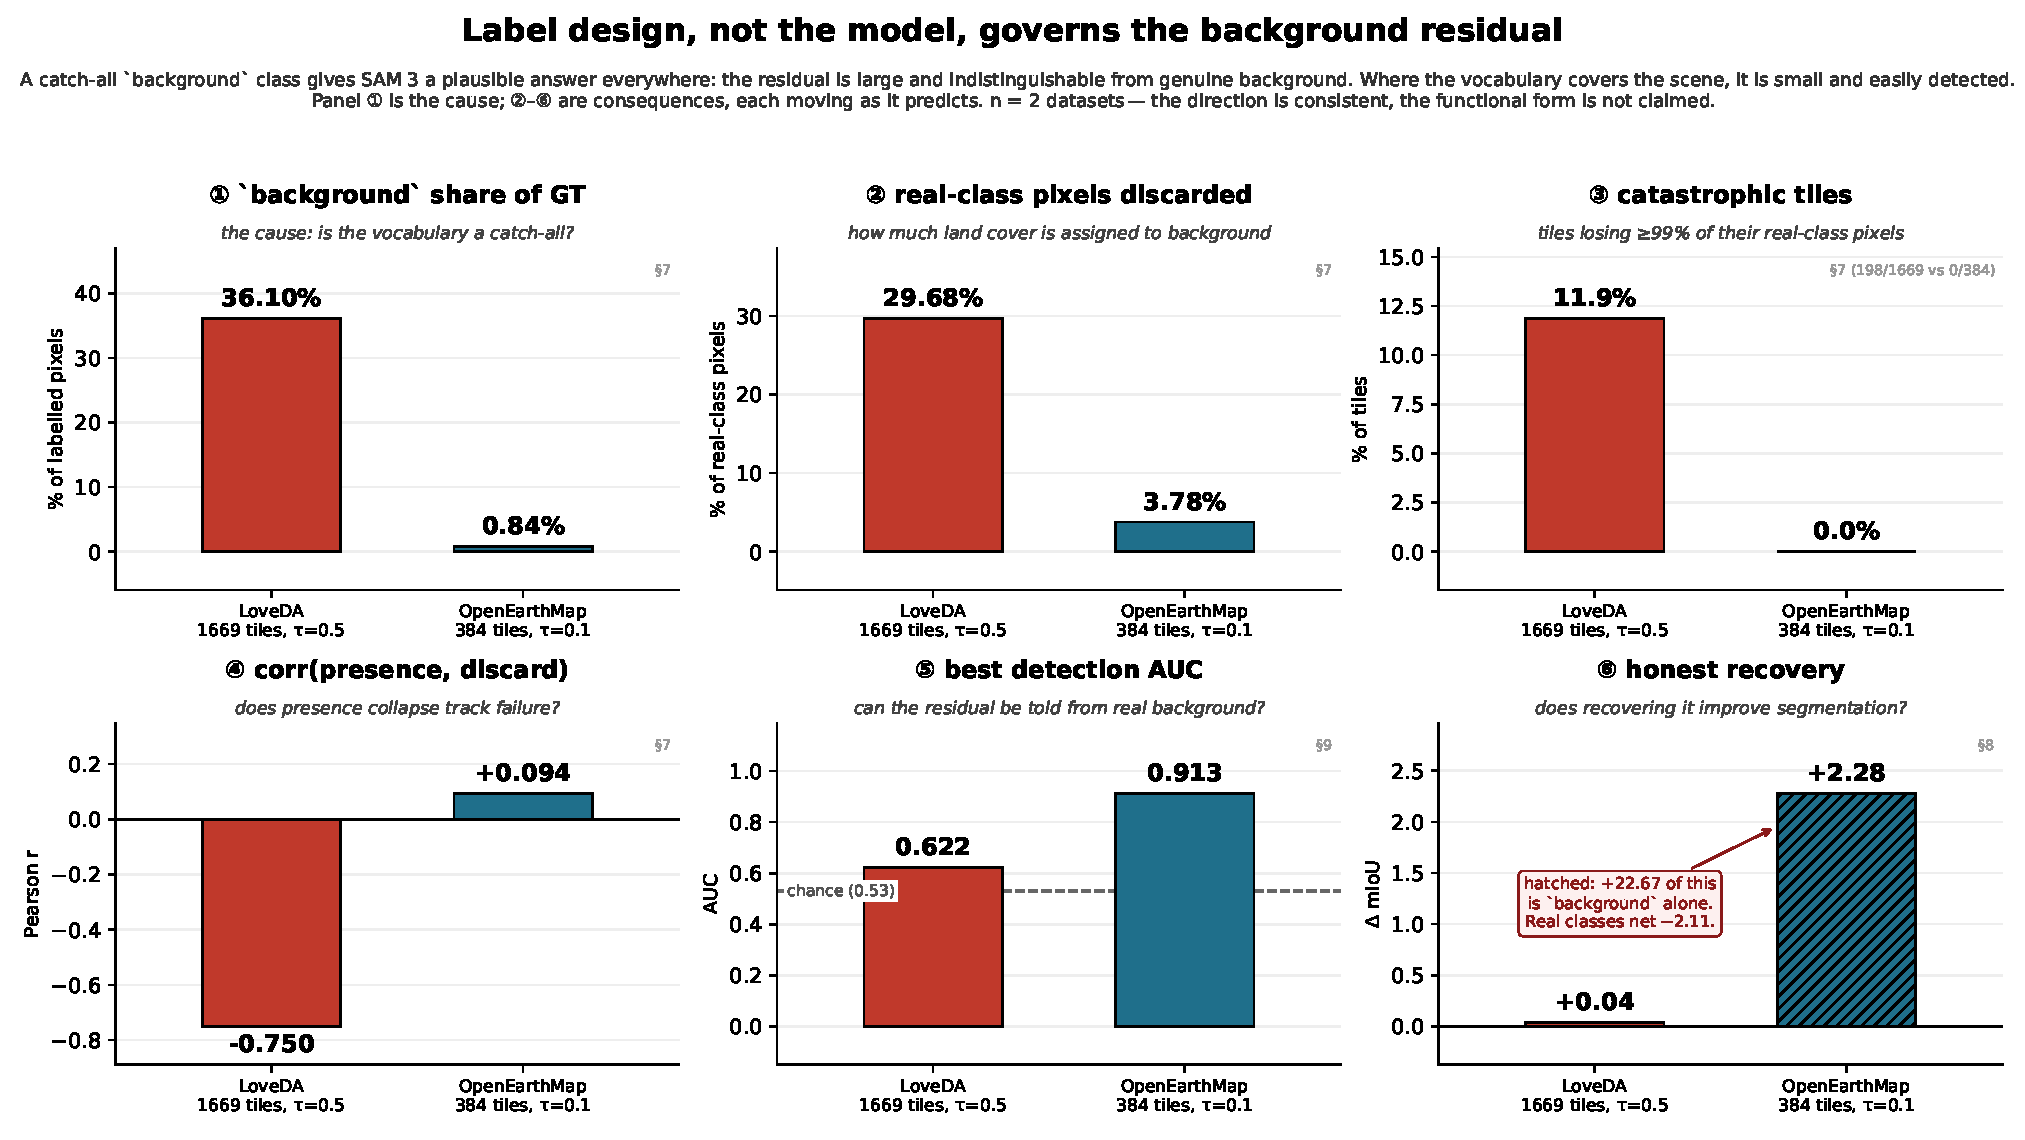
\includegraphics[width=\textwidth]{fig2_mechanism.pdf}
\caption{The residual's size, its detectability, and the presence-score correlation
all move with the catch-all class's share of ground truth. The mechanism is
established by intervention, not correlation: because that share is set by the
vocabulary, we manipulate it directly with class count controlled.}
\label{fig:mechanism}
\end{figure*}

\begin{table}[t]\centering\small
\caption{The residual is ordered by the catch-all's share of ground truth, across
four datasets. The Potsdam row was predicted from ground-truth masks alone and
registered before the pipeline was run.}
\label{tab:cmech}
\begin{tabular}{lrr}
\toprule
 & catch-all share & real-class pixels discarded \\
\midrule
OpenEarthMap & \bgShareOEM{} & \discardOEM{} \\
Potsdam      & \potsShare{} & \potsDiscard{} \\
UAVid        & \uavCatchShare{} & \uavDiscard{} \\
LoveDA       & \bgShareLove{} & \discardPct{} \\
\bottomrule
\end{tabular}
\end{table}

How much real land cover a presence-gated pipeline discards is not a property of the
model. It is ordered by how much of the scene the dataset's catch-all class covers
(Table~\ref{tab:cmech}). A catch-all gives the model a plausible answer everywhere, so
a strong runner-up carries no information: on LoveDA nine tested signals reach a best
AUC of \aucLove{} against a \aucFloor{} floor, while on OpenEarthMap the runner-up
score separates the residual at \aucOEM{}.

Because the catch-all's share is set by the \emph{vocabulary}, we can intervene on it
rather than stratify. Merging real classes into the catch-all at increasing doses,
against a control that merges the same classes into \emph{each other} so class count
moves identically, drives detectability \ivAtwo{}~$\to$~\ivBtwo{} while the control
moves only to \ivDtwo{} (\suppref{sec:dose}). A second arm localises the effect to the
label space rather than the prompt list.

\paragraph{Recovery is not the answer.} Having measured the residual, we tried to
recover it and report the failure: a region-level labeller reaches \recoverLove{}~mIoU
on LoveDA, and its apparent \recoverOEM{} on OpenEarthMap is entirely the catch-all
ceasing to be over-predicted (\oemBgGain{}~IoU) while the real classes lose
\oemRealLoss{}. \best{The residual is real and recovering it after the fact does not
work.} What does work is not making the decision wrongly in the first place.

% =====================================================================
\section{Two levers}
\label{sec:method}

\paragraph{Lever one: a threshold per class.} The baseline predicts
$\hat{c} = \arg\max_c s_c$ and emits \bg{} when $s_{\hat c} < \tau$. We replace the
scalar with a vector: emit \bg{} when $s_{\hat c} < \tau_{\hat c}$. Nothing else
changes, and with a constant vector the rule is bit-identical to the baseline.

\best{This is the complete family of corrections available after the argmax.} Let
$g_c$ be any per-class strictly monotone map applied to the scores, followed by a
global threshold $t$. Because $g_c$ is monotone, $g_c(s) \geq t$ holds exactly when
$s \geq g_c^{-1}(t)$, so the composition is the per-class rule with
$\tau_c = g_c^{-1}(t)$. Any post-argmax recalibration --- temperature, vector scaling,
isotonic --- therefore reduces to choosing $\tau_c$, and cannot beat choosing it
directly.

\paragraph{The objective separates, so the fit is exact.} For a fixed argmax, a pixel
predicted $c$ either clears $\tau_c$ or becomes the catch-all; it can never become a
different real class. So $\mathrm{TP}_c$, $\mathrm{FP}_c$ and $\mathrm{FN}_c$ depend
on $\tau_c$ alone and the real-class objective is a sum of single-variable terms.
Coordinate ascent is therefore \best{exact rather than greedy} --- one sweep per class
is the global optimum --- and costs $N \times 201$ evaluations rather than $201^N$. We
verify this at exactly $\sepExact{}$ over \sepSweeps{} class sweeps on three datasets.

\paragraph{Lever two: a multiplier before the argmax.} The completeness result holds
only \emph{given} the argmax, which points at the remaining freedom. We predict
$\hat{c} = \arg\max_c w_c s_c$ and keep the pixel when $s_{\hat c} \geq \tau_{\hat c}$
--- \best{the argmax reads the scaled score, the threshold reads the raw one}. That
asymmetry is what confines $w$ to the decision: a scale applied after the argmax would
be monotone and merely reparameterise $\tau$. Only ratios of $w$ matter, so we
renormalise to geometric mean one after each pass. $(w, \tau)$ are fitted jointly on
the same tiles, and nothing is trained.

This reaches a mass no threshold can. A pixel whose correct class \emph{lost} the
argmax is not below that class's bar --- it is behind another class --- and lowering
its threshold returns it wearing the wrong label.

% =====================================================================
\section{Results}
\label{sec:results}

\begin{figure*}[t]\centering
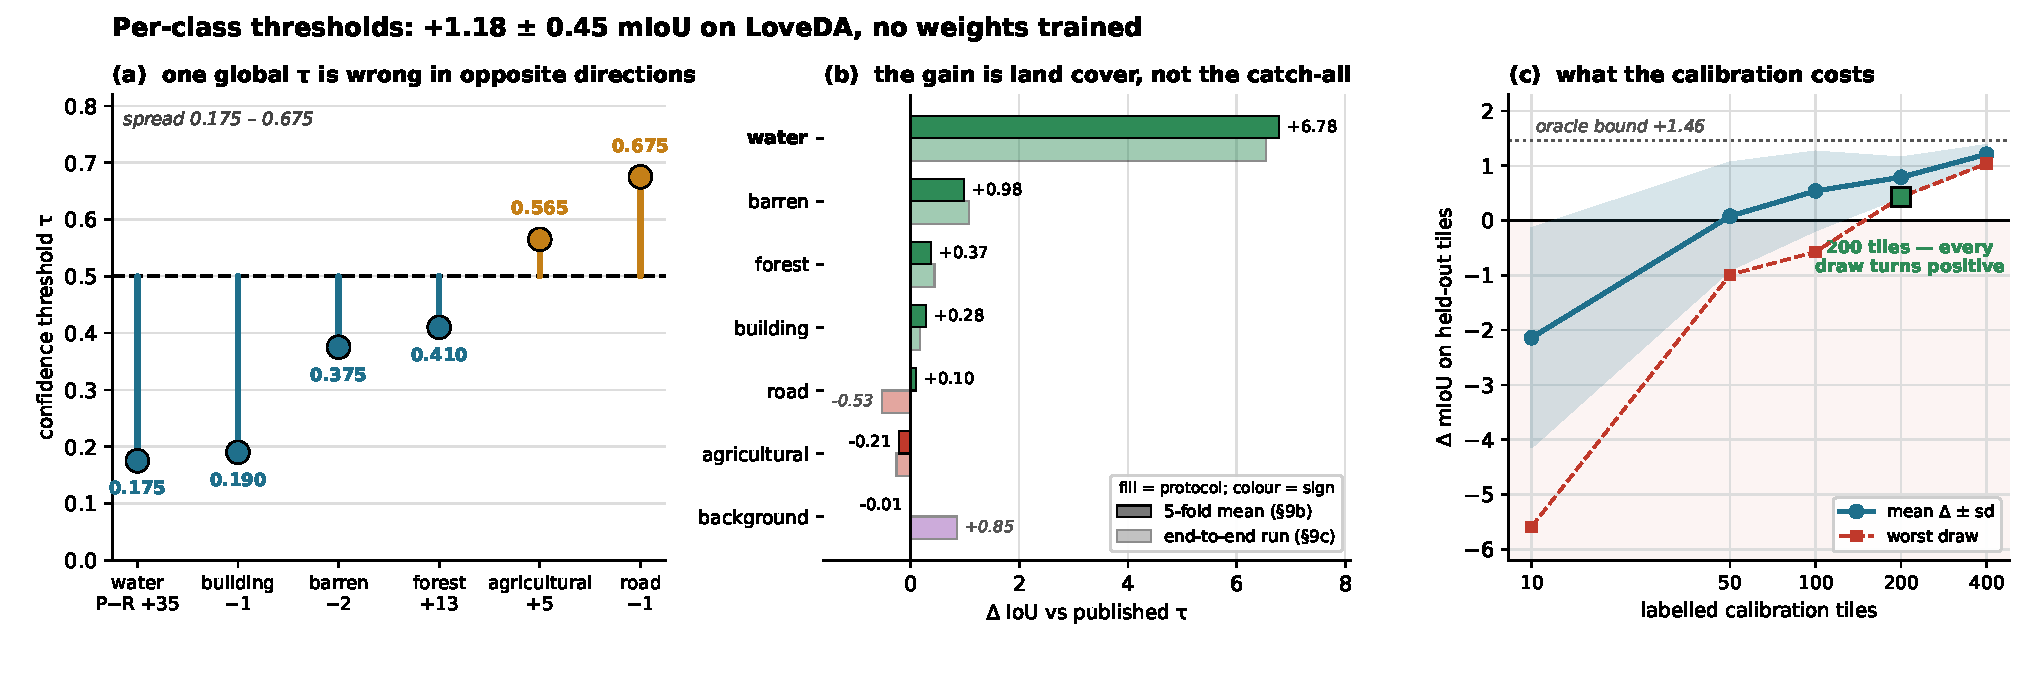
\includegraphics[width=\textwidth]{fig7_method.pdf}
\caption{Left: fitted thresholds against the single published value. Centre:
per-class IoU change. Right: the calibration curve --- the gain is reliably positive
from roughly \calibTiles{} tiles on LoveDA, and from \uavCalibScenes{} flights on
UAVid.}
\label{fig:method}
\end{figure*}

\begin{table}[t]\centering\small
\caption{Both levers, across four datasets and a second pipeline. $\Delta$ is over
the published threshold on identical held-out pixels. Catch-all-excluded mIoU is
reported beside the headline throughout, for the reason in
Sec.~\ref{sec:results}.}
\label{tab:cmain}
\begin{tabular}{lrrr}
\toprule
 & lever 1 & lever 2 & excl.\ catch-all \\
\midrule
LoveDA        & \best{\methodGain{}} & \best{\scLove{}} & \methodLandMean{} / \scLoveExcl{} \\
Potsdam       & \potsFull{} & \best{\scPots{}} & \potsReal{} \\
UAVid         & \best{\uavTauCV{}} & \best{\uavScaleCV{}} & --- \\
OpenEarthMap  & \oemTauCV{} & --- & \best{\mrOemReal{}} \\
\midrule
ConInfer (CLIP) & \best{\cnCV{}} & \scCI{} & \cnReal{} \\
\bottomrule
\end{tabular}
\end{table}

\paragraph{Thresholds.} Five-fold cross-validation gives
\methodGain{}~$\pm$~\methodSD{}~mIoU on LoveDA with every fold positive and a worst
fold of \methodWorst{}, capturing \oracleShare{} of an oracle bound of
\oracleBound{}. The gain is entirely land cover: the catch-all moves \methodBg{}~IoU.
It is driven by \texttt{water}, which gains \methodWater{}~IoU alone at a fitted
threshold of \methodWaterTau{} against a global $\tauLove{}$. \best{The headroom is smaller
than it looks, which makes the gain larger than it looks}: a fully supervised
SegFormer-b0 trained on the whole LoveDA training set reaches \oracleSup{}, so
\best{\gapClosed{} of the gap between training-free and fully supervised is closed by
\calibTiles{} labelled tiles and no trained weights}.

\paragraph{It is not backbone-specific, but it is dataset-specific.} Applied unchanged
to ConInfer at \emph{its} published operating point, the same rule adds
\cnCV{}~$\pm$~\cnCVsd{} on LoveDA with every fold positive and every class improving
--- \best{so our method composes with the nearest published competitor rather than
beating it}, taking its reproduction from \cnRepro{} to \cnFit{}. On OpenEarthMap it
helps neither pipeline's headline, for the same reason in both: the fit must sacrifice
a catch-all sitting at \mrOemBgIoU{}~IoU that owns a ninth of the metric.

\paragraph{The scale reaches what thresholds cannot.} It adds \scPots{} on Potsdam,
\scLove{} on LoveDA and \uavScaleCV{} on UAVid over thresholds alone. Potsdam's
\texttt{tree} is the clean case: the largest precision--recall gap we measure
(\treeGap{}), which per-class thresholds move \treeTau{} and the scale moves
\best{\treeScale{}}. The reason is measurable --- \texttt{tree}'s residual is
\emph{below} the threshold but with a \emph{different class} winning the argmax, so
lowering its own threshold returns those pixels mislabelled.

\begin{figure}[t]\centering
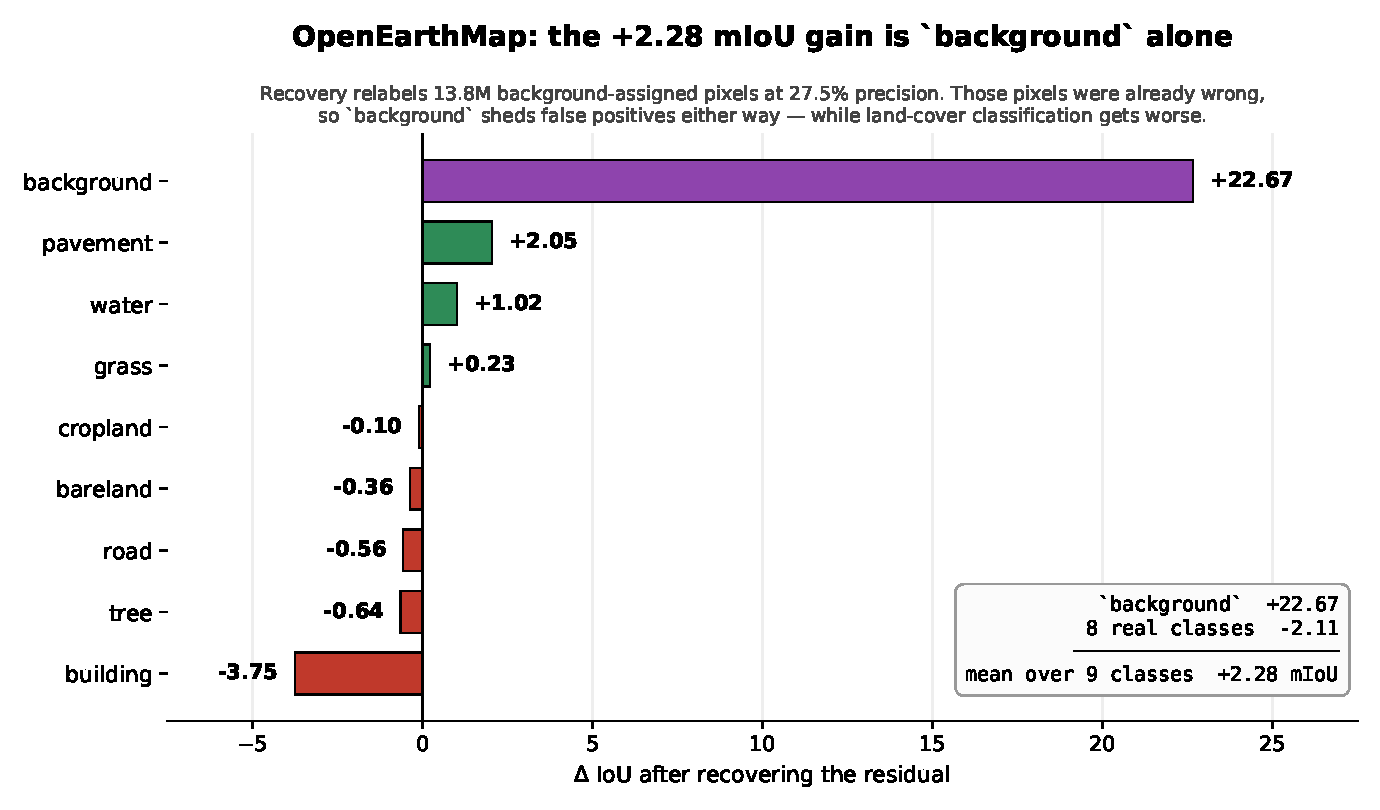
\includegraphics[width=\columnwidth]{fig3_oem_per_class.pdf}
\caption{A headline mIoU gain that is not a segmentation improvement: the catch-all
supplies \oemBgGain{}~IoU while the real classes lose \oemRealLoss{}. We observe the
same artefact with the opposite sign elsewhere, which is why we treat it as a property
of the metric.}
\label{fig:oemperclass}
\end{figure}

\paragraph{Report both metrics.} mIoU is an \emph{unweighted} mean over $N$ classes,
so \best{a catch-all owns exactly $1/N$ of the score however meaningful it is} ---
\mrOemLever{} on OpenEarthMap for a class covering \bgShareOEM{} of the pixels. We
observe that class moving the headline in both directions: supplying
\oemBgGain{}~IoU of an apparent gain in one experiment (Fig.~\ref{fig:oemperclass})
and cancelling a real one in another. The distortion exists before any method is
applied --- OpenEarthMap's published headline is depressed \mrOemDistort{} points by
that single class --- so we report mIoU over the real classes beside the headline, and
suggest the field does.

\paragraph{The correction reaches the residual the paper opened with.} Held out, it
lowers the discard rate \raDiscA{}~$\to$~\raDiscC{}, and \best{\raCorrect{} of the
pixels it recovers land on the correct class --- \raWPR{} wrong per right, against
\tauRatio{} for the global threshold sweep that reaches the same mass.}

\paragraph{UAVid, and a correction to our own headline.} On drone video both levers
hold under flight-grouped folds and transfer across the split boundary: fitted on the
training split and applied unchanged, they take \uavBase{} to \uavEEone{} and then to
\best{\uavEEtwo{}}, verified in the unmodified pipeline against a cached prediction of
\uavEEpred{} --- exact on the headline, every class within \uavEEmax{}. Pixel accuracy
rises \uavaAccA{}~$\to$~\uavaAccC{} and mean precision and recall \emph{both} rise
(\uavPrecD{}, \uavRecD{}). \best{We then found that most of the scale's gain there was
repairing a word}, and restate the contribution accordingly in the next section.

% =====================================================================
\section{A larger lever than either, and no rule for setting it}
\label{sec:vocab}

\begin{table}[t]\centering\small
\caption{The same rule --- use the dataset's own class name --- applied to the same
class, on two datasets. One word changes; prompt count per class does not.}
\label{tab:cvocab}
\begin{tabular}{llll}
\toprule
 & shipped & annotation guide & $\Delta$ mIoU \\
\midrule
UAVid   & \texttt{vegetation} & \emph{low vegetation} & \best{\vocUavGain{}} \\
Potsdam & \texttt{grass}      & \emph{low vegetation} & \best{\vocPotsGain{}} \\
\bottomrule
\end{tabular}
\end{table}

\begin{figure*}[t]\centering
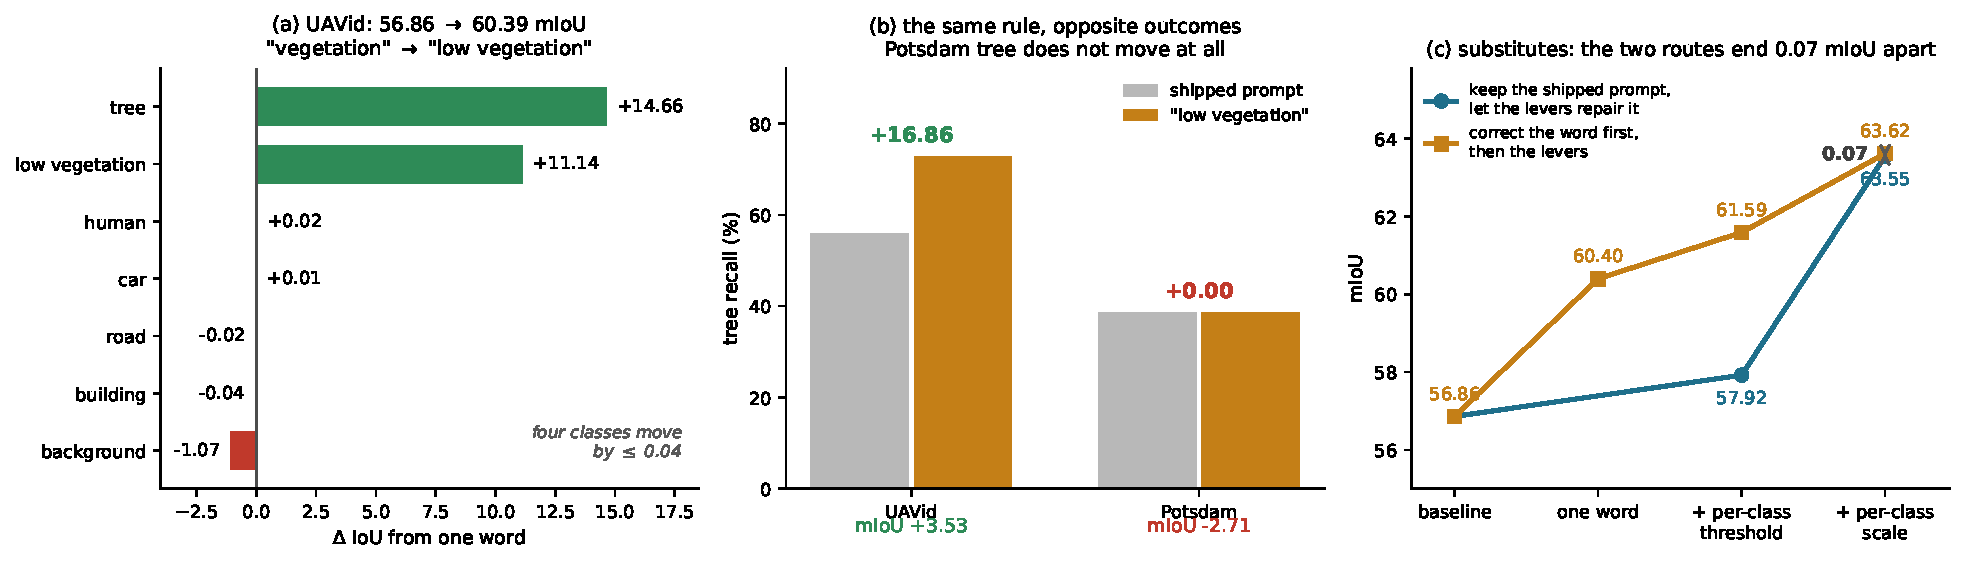
\includegraphics[width=\textwidth]{fig11_vocab_lever.pdf}
\caption{One word against the whole method. \textbf{(a)} On UAVid the correction is surgical: two classes move, four move by at most \vocUavElse{}. \textbf{(b)} The same rule on Potsdam \emph{costs} mIoU, and \texttt{tree}'s recall does not move at all --- the two datasets present identically in a results table and have different causes. \textbf{(c)} The word and the multiplier are substitutes: correcting the prompt first, or leaving it and letting both levers repair it, end \vocRouteDelta{}~mIoU apart.}
\label{fig:vocab}
\end{figure*}

Every training-free open-vocabulary method inherits a hand-written list of class
prompts, and none of the work we compare against reports how that list was chosen.
Our own results above are stated at a vocabulary we did not write. We therefore
tested it on two datasets, with the prediction committed to version control before
each run.

\paragraph{On UAVid one word is worth \vocUavGain{}~mIoU, and it is surgical.}
\texttt{tree} gains \vocUavTree{} and the low-vegetation class \vocUavVeg{}, while
\best{every other real class moves by at most \vocUavElse{}}. The mechanism appears in
the two quantities we registered in advance: the shipped \texttt{vegetation} was
firing on anything green, and its precision rises
\vocUavVegPrecA{}~$\to$~\vocUavVegPrecB{}; \texttt{tree} was losing those pixels, and
its recall rises \vocUavTreeRecA{}~$\to$~\vocUavTreeRecB{}.

\paragraph{On Potsdam the identical rule \best{costs} \vocPotsGain{}~mIoU.} We
registered that the change would move the score by less than a point and were wrong
about the magnitude. The shipped \texttt{grass} is \emph{better} than the official
term: specific, visual, and crucially it does not name the neighbouring class. \best{So
the annotation guide's own wording is not automatically the better prompt.}

\paragraph{The prediction that did hold identifies the mechanism.} Potsdam's
\texttt{tree} recall is \vocPotsTreeRec{} before the change and \vocPotsTreeRec{}
after --- unchanged to a hundredth --- while its precision falls
\vocPotsTreePrecA{}~$\to$~\vocPotsTreePrecB{} as the weaker prompt leaks pixels into
it. \best{Renaming a competing class changes nothing about \texttt{tree} there.} Its
deficit is visual confusion at 5\,cm ground sampling distance, not a naming error,
which is why the scale reaches it and a better word does not. \best{The two datasets
present identically in the results table --- a scale gain carried by \texttt{tree} ---
and have different causes.}

\paragraph{The word and the multiplier are substitutes.} On UAVid the two routes end
in the same place: keeping the flawed prompt and letting both levers repair it reaches
\vocRouteA{}, while correcting the word first and then applying both levers reaches
\vocRouteB{} --- \vocRouteDelta{}~mIoU apart, and within about a point per class.
\best{Typing two words and fitting a multiplicative reweighting on \uavTrainTiles{}
labelled frames address the same pixels.} One class does not substitute:
\texttt{human} gains the same either way, because it is not losing an argmax to a
mis-named neighbour, it is simply too conservative.

\paragraph{We therefore restate our own result.} Correcting the word removes
\uavScaleLost{} of the scale's gain on UAVid (\uavScaleTrans{}~$\to$~\uavCorrTwo{}),
so that dataset's method contribution is \best{\uavCorrMethod{}} --- \uavCorrOne{}
from thresholds and \uavCorrTwo{} from the scale on a corrected baseline of
\uavCorrBase{}, reaching \uavCorrFinal{}. That is in line with \loveTotal{} on LoveDA
and \potsTotal{} on Potsdam.

\paragraph{What we take from this.} A one-word change is worth \vocUavGain{} on UAVid
and \vocLoveBarren{} on LoveDA, against \loveTotal{} for our complete method on
LoveDA. \best{The vocabulary is the largest single lever we measure, it is unreported,
and the direction of a change to it is not predictable from the class name.} We do not
offer a method for choosing prompts --- our two arms disagree, which is the point. We
offer the measurement, and the recommendation that prompt lists be reported and
ablated alongside the architecture, because on these benchmarks they are worth more
than the methods being compared.

% =====================================================================
\section{Why the calibration set is irreducible}
\label{sec:bound}

The method costs \calibTiles{} labelled tiles. It is natural to ask whether a
label-free rule could choose the thresholds instead, and we tried \nAttempts{} ---
Otsu splits, confidence percentiles, presence-scaled thresholds, cross-head agreement,
and others. None reaches the oracle bound; on LoveDA every one scores \emph{below} the
published threshold.

\best{The instructive part is why.} We had supposed the missing quantity was per-class
precision, which is label-derived by definition. It is not: four of the label-free
statistics predict per-class precision at Spearman $\rho \geq \proxyRho{}$ with exact
$p \leq \proxyP{}$, and they still buy nothing. Precision does not determine the
threshold, and the relation is not even monotone --- \texttt{water} at $\bndWaterPrec{}\%$
precision takes the \emph{lowest} threshold while \texttt{road} at $\bndRoadPrec{}\%$ takes the
\emph{highest}.

The real bound is structural. The optimal threshold vector solves a \emph{coupled}
multi-class objective: raising one class's threshold pushes pixels into the catch-all,
changing every other class's optimum. No per-class scalar can express that, measurable
or not. \best{That is why a six-parameter fit works and every one-parameter rule
fails}, and it generalises to any training-free pipeline that thresholds a per-class
score.

% =====================================================================
\section{Limitations}
\label{sec:limitations}

\paragraph{\best{Our remaining results are stated at vocabularies we have not
audited.}} Sec.~\ref{sec:vocab} shows one word is worth more than our complete method
on LoveDA and that the direction of such a change is unpredictable. We tested two
prompts on two datasets. LoveDA's and OpenEarthMap's lists are untested by the same
rule and we cannot exclude that part of their reported gains is available by
rewording. Two things bound this rather than excuse it: Potsdam was tested
\emph{because} its scale gain has UAVid's signature and came back clean, and LoveDA's
list already carries hand-tuned synonyms whose removal costs \vocLoveBarren{}~mIoU.
Neither substitutes for auditing it.

\paragraph{One reproduction does not reproduce.} Our UAVid baseline is \uavGap{} above
the published figure under identical code, configuration, vocabulary and thresholds,
and their released configuration points at a split whose labels are not public. We
quote gains against our own reproduction throughout, as we do in the opposite
direction for ConInfer, whose LoveDA figure we reproduce \cnGap{} \emph{below} its
published value. A difference measured on one pipeline is robust to a constant offset
in it; an absolute comparison across two is not, and we do not make one.

\paragraph{Thresholds do not transfer across a domain shift.} Fitted on LoveDA's rural
tiles and applied to urban ones they land \emph{below} the published threshold. The
calibration set must match the evaluation distribution, and pooling across two
distributions reproduces the failure of the global threshold one level up. We find one
label-free predictor of when transfer will work --- agreement in discard rate between
source and target, which orders four split pairs --- but four points across two
datasets is an ordering, not a law.

\paragraph{Seventy frames from seven flights is a sample of seven.} UAVid's validation
split is video, so its effective sample size is the flight count; a five-fold inside it
has a baseline that swings eighteen mIoU points across folds. We fit on the training
split and evaluate on validation whole for that reason. The same caution applies to any
video-derived benchmark evaluated with frame-level splits.

\paragraph{The negative results are ours too.} Three further per-class corrections ---
fusing the two SAM~3 heads, weighting the presence score, and affine rather than
diagonal scaling --- were fitted under the same protocol and gate, and all three are
null (\suppref{sec:levers}). Each was pre-registered as a small positive.

% =====================================================================
\section{Conclusion}
\label{sec:conclusion}

A single confidence threshold is the wrong shape for a multi-class open-vocabulary
decision. Fitting one per class, and one multiplier per class before the argmax,
recovers a consistent gain across four datasets and two backbones on the supervision
the baseline already spends --- and the first of those two rules is provably
everything available after the argmax. But the largest lever we found is not ours: the
hand-written prompt list that every method in this literature inherits and none
reports is worth more, on these benchmarks, than the methods being compared. We
recommend it be reported.

{\small
\bibliographystyle{plain}
\bibliography{refs}
}

\end{document}
